\documentclass{article}
\usepackage[utf8]{inputenc}
\usepackage[margin=1in]{geometry}
\usepackage{tikz}
\usetikzlibrary{shapes.geometric, arrows.meta, positioning, calc}

\begin{document}

\begin{figure}[htbp]
\centering
\resizebox{\textwidth}{!}{
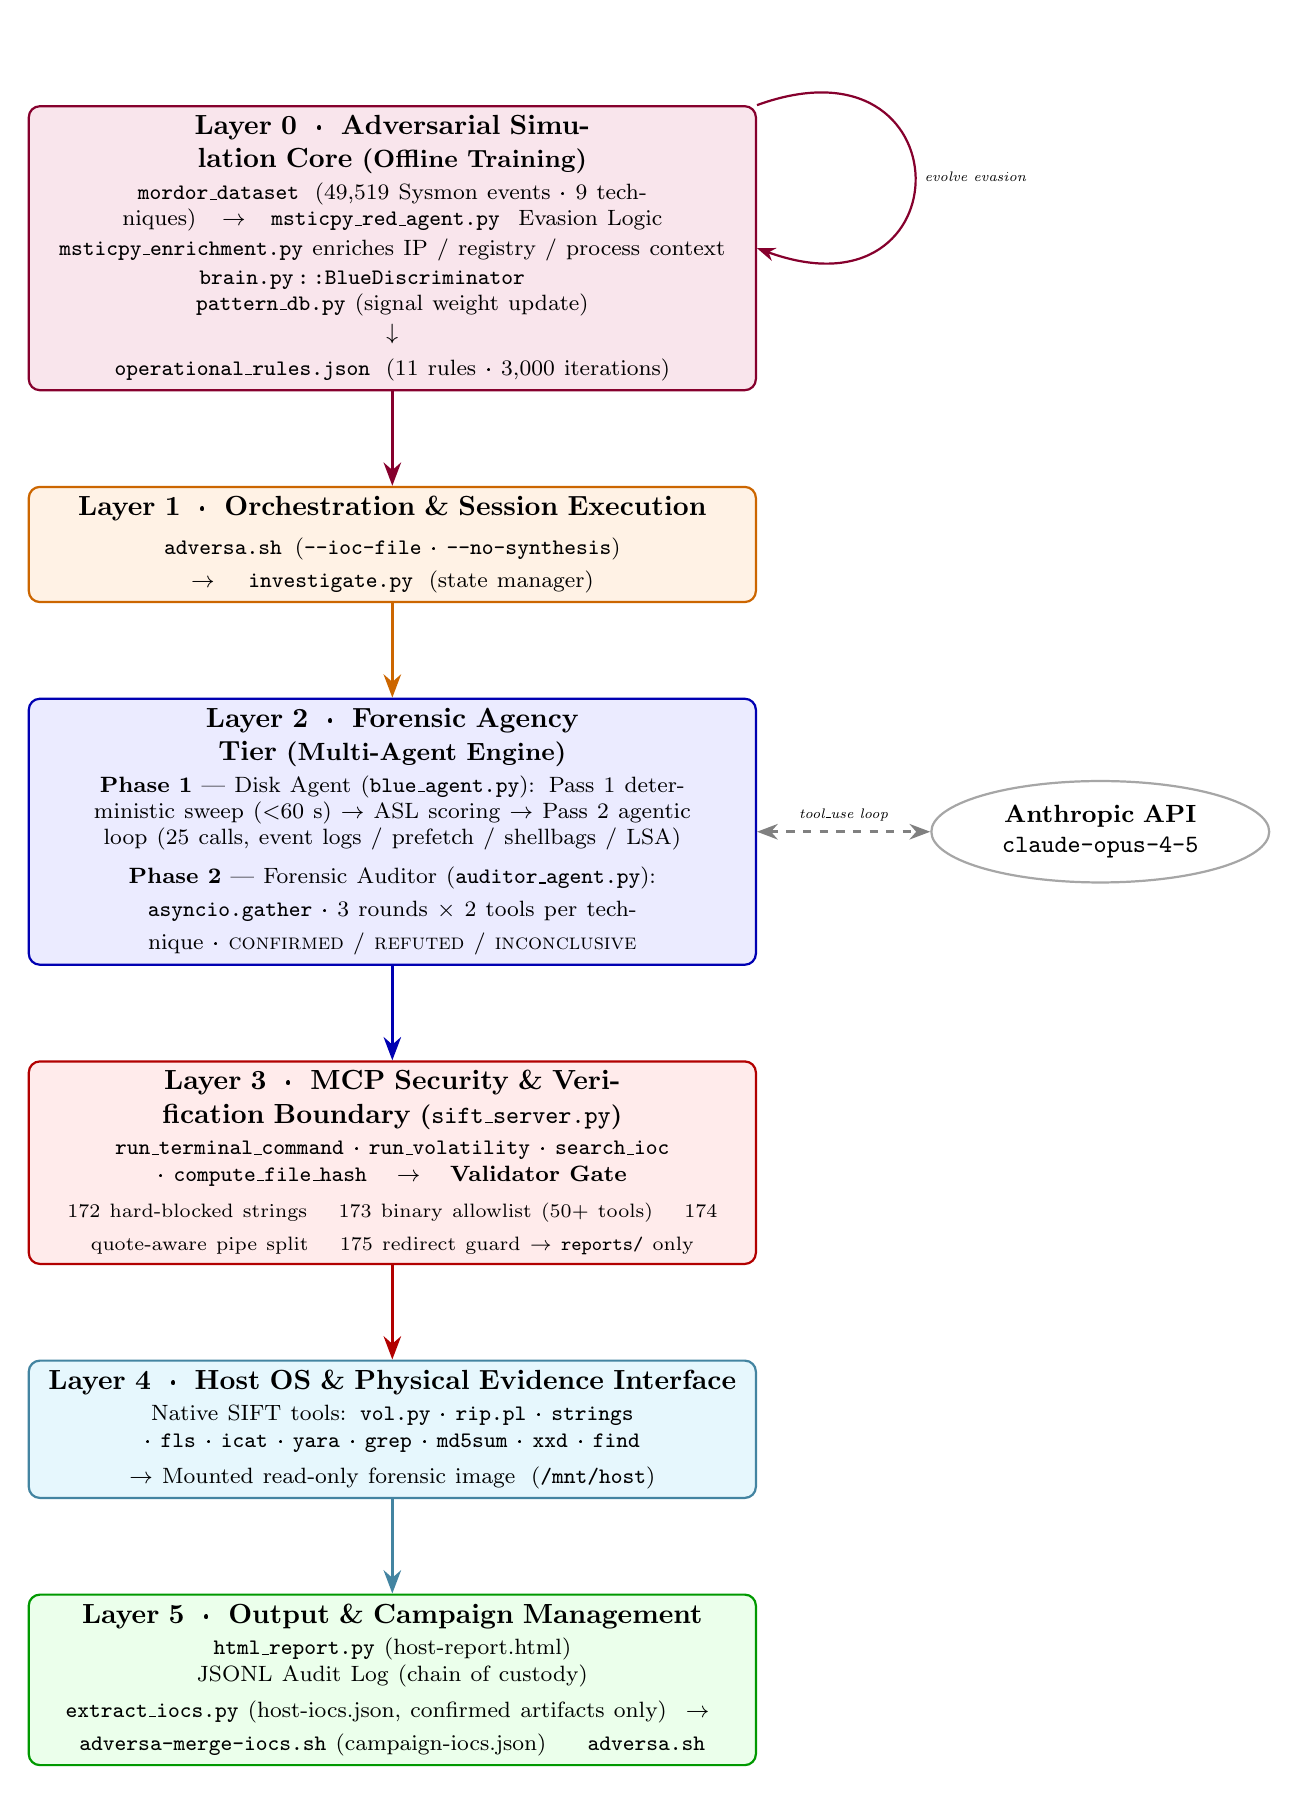
\begin{tikzpicture}[
    node distance=1.2cm,
    auto,
    >=Stealth,
    layer/.style={
        rectangle, draw=black, thick, fill=#1,
        text width=9cm, minimum height=1.4cm,
        align=center, rounded corners
    },
    api/.style={
        ellipse, draw=gray!70, fill=white, thick,
        text width=2.8cm, align=center, font=\small
    },
    arrow/.style={->, thick, line width=1.2pt}
]

    %% ── LAYER 0 ──────────────────────────────────────────────────
    \node (L0) [layer=purple!10, draw=purple!70!black] {
        \textbf{Layer 0 \;·\; Adversarial Simulation Core \small(Offline Training)} \\[2pt]
        \footnotesize
        \texttt{mordor\_dataset} \;(49{,}519 Sysmon events · 9 techniques)
        $\;\rightarrow\;$
        \texttt{msticpy\_red\_agent.py} $\rightleftarrows$ Evasion Logic \\[1pt]
        \texttt{msticpy\_enrichment.py} enriches IP / registry / process context \\[1pt]
        \texttt{brain.py\,:\,:BlueDiscriminator}
        $\;\rightleftarrows\;$
        \texttt{pattern\_db.py} (signal weight update) \\[1pt]
        $\downarrow$ \\[1pt]
        \texttt{operational\_rules.json} \;(11 rules · 3{,}000 iterations)
    };

    %% Self-loop arrow for evasion evolution
    \draw[->, thick, draw=purple!70!black]
        (L0.north east)
        to [out=20, in=340, looseness=4]
        node[right, font=\tiny\itshape] {evolve evasion}
        (L0.east);

    %% ── LAYER 1 ──────────────────────────────────────────────────
    \node (L1) [layer=orange!10, draw=orange!80!black, below=of L0] {
        \textbf{Layer 1 \;·\; Orchestration \& Session Execution} \\[2pt]
        \footnotesize
        \texttt{adversa.sh}
        \,(\texttt{-{}-ioc-file} · \texttt{-{}-no-synthesis})
        $\;\rightarrow\;$
        \texttt{investigate.py} \;(state manager)
    };

    %% ── LAYER 2 ──────────────────────────────────────────────────
    \node (L2) [layer=blue!8, draw=blue!70!black, below=of L1] {
        \textbf{Layer 2 \;·\; Forensic Agency Tier \small(Multi-Agent Engine)} \\[2pt]
        \footnotesize
        \textbf{Phase 1} — Disk Agent (\texttt{blue\_agent.py}):
            Pass 1 deterministic sweep ($<$60 s)
            $\rightarrow$ ASL scoring
            $\rightarrow$ Pass 2 agentic loop (25 calls, event logs / prefetch / shellbags / LSA) \\[2pt]
        \textbf{Phase 2} — Forensic Auditor (\texttt{auditor\_agent.py}):
            \texttt{asyncio.gather} · 3 rounds $\times$ 2 tools per technique ·
            \textsc{confirmed} / \textsc{refuted} / \textsc{inconclusive}
    };

    %% Anthropic API node (right of L2)
    \node (API) [api, right=2.2cm of L2] {
        \textbf{Anthropic API} \\
        \small\texttt{claude-opus-4-5}
    };

    %% ── LAYER 3 ──────────────────────────────────────────────────
    \node (L3) [layer=red!8, draw=red!70!black, below=of L2] {
        \textbf{Layer 3 \;·\; MCP Security \& Verification Boundary
            \small(\texttt{sift\_server.py})} \\[2pt]
        \footnotesize
        \texttt{run\_terminal\_command} · \texttt{run\_volatility} ·
        \texttt{search\_ioc} · \texttt{compute\_file\_hash}
        $\;\rightarrow\;$ \textbf{Validator Gate} \\[1pt]
        \scriptsize
        \ding{172} hard-blocked strings \quad
        \ding{173} binary allowlist (50+ tools) \quad
        \ding{174} quote-aware pipe split \quad
        \ding{175} redirect guard $\rightarrow$ \texttt{reports/} only
    };

    %% ── LAYER 4 ──────────────────────────────────────────────────
    \node (L4) [layer=cyan!10, draw=cyan!60!black, below=of L3] {
        \textbf{Layer 4 \;·\; Host OS \& Physical Evidence Interface} \\[2pt]
        \footnotesize
        Native SIFT tools:
        \texttt{vol.py} · \texttt{rip.pl} · \texttt{strings} · \texttt{fls} · \texttt{icat} ·
        \texttt{yara} · \texttt{grep} · \texttt{md5sum} · \texttt{xxd} · \texttt{find} \\[1pt]
        $\rightarrow$ Mounted read-only forensic image \;(\texttt{/mnt/host})
    };

    %% ── LAYER 5 ──────────────────────────────────────────────────
    \node (L5) [layer=green!8, draw=green!60!black, below=of L4] {
        \textbf{Layer 5 \;·\; Output \& Campaign Management} \\[2pt]
        \footnotesize
        \texttt{html\_report.py} (host-report.html) \quad
        JSONL Audit Log (chain of custody) \\[1pt]
        \texttt{extract\_iocs.py} (host-iocs.json, confirmed artifacts only)
        $\;\rightarrow\;$
        \texttt{adversa-merge-iocs.sh} (campaign-iocs.json)
        $\;\dashrightarrow\;$
        \texttt{adversa.sh}
    };

    %% ── VERTICAL FLOW ────────────────────────────────────────────
    \draw [arrow, draw=purple!70!black] (L0) -- (L1);
    \draw [arrow, draw=orange!80!black] (L1) -- (L2);
    \draw [arrow, draw=blue!70!black]   (L2) -- (L3);
    \draw [arrow, draw=red!70!black]    (L3) -- (L4);
    \draw [arrow, draw=cyan!60!black]   (L4) -- (L5);

    %% ── API HANDSHAKE ────────────────────────────────────────────
    \draw [<->, dashed, line width=1pt, draw=gray]
        (L2.east) -- (API.west)
        node[midway, above, font=\tiny\itshape] {tool\_use loop};

\end{tikzpicture}
}
\caption{AdversA Layered Forensic Architecture Stack}
\label{fig:adversa_architecture}
\end{figure}

\end{document}
